% !TeX root = Gruppe_0-projektrapport.tex


\documentclass[12pt]{article}
\usepackage{lingmacros}
\usepackage{tree-dvips}
\usepackage[utf8]{inputenc}
\usepackage{fancyhdr}
\usepackage{listings}
\usepackage{subfig}
\usepackage{xcolor}
\usepackage{geometry}
\usepackage{pdflscape}

\usepackage{float}
\geometry{
a4paper,
total={170mm,257mm},
left=15mm,
top=20mm,
}
\usepackage{graphicx}
\usepackage{wrapfig}
\usepackage{amsmath}
\usepackage{hyperref}
\definecolor{link}{rgb}{0,0,215}
\hypersetup{
    colorlinks=true,
    linkcolor=link,
    filecolor=link,      
    urlcolor=link,
    pdfpagemode=FullScreen,
}

\graphicspath{ {./img} }

\definecolor{comment}{rgb}{0,0.45,0}
\definecolor{codegray}{rgb}{0.5,0.5,0.5}
\definecolor{codepurple}{rgb}{0.58,0,0.82}
\definecolor{backcolour}{rgb}{0.95,0.95,0.92}
\lstdefinestyle{CodeStyle}{
    backgroundcolor=\color{backcolour},   
    commentstyle=\color{comment},
    keywordstyle=\color{magenta},
    numberstyle=\tiny\color{codegray},
    stringstyle=\color{codepurple},
    basicstyle=\ttfamily\footnotesize,
    breakatwhitespace=false,         
    breaklines=true,                 
    captionpos=b,                    
    keepspaces=true,                 
    numbers=left,                    
    numbersep=5pt,                  
    showspaces=false,                
    showstringspaces=false,
    showtabs=false,                  
    tabsize=2
}
\lstset{style=CodeStyle}
\lstdefinelanguage{JavaScript}{
  keywords={typeof, new, true, false, catch, function, return, null, catch, switch, var, if, in, while, do, else, case, break},
  keywordstyle=\color{purple}\bfseries,
  ndkeywords={class, export, const, var, let, boolean, throw, implements, import, this, !!, !=, ===, ;},
  ndkeywordstyle=\color{blue}\bfseries,
  identifierstyle=\color{black},
  sensitive=false,
  comment=[l]{//},
  morecomment=[s]{/*}{*/},
  commentstyle=\color{comment}\ttfamily,
  stringstyle=\color{orange}\ttfamily,
  morestring=[b]',
  morestring=[b]"
}

%%%%%%% Document begin %%%%%%%%%%%
\begin{document}
\begin{titlepage}
    \centering

    \vspace*{1cm}

    % Title and subtitle are enclosed between two rules.
    \rule{\textwidth}{1pt}

    % Title
    \vspace{.7\baselineskip}
    {\huge \textbf{Miniature World}}

    % Subtitle
    \vspace*{.5cm}
    {\LARGE Digitalt Økosystem, 1. Semesterprojekt}
    
    \rule{\textwidth}{1pt}

    \vspace{1cm}

    % Set this size for the remaining titlepage.
    \large

    % Authors side by side, using two minipages as a trick.
    \begin{minipage}{.5\textwidth}
        \centering
        Johannes Gunge Jørgensen \\
        {\normalsize \url{jgjo@itu.dk}}
    \end{minipage}%
    \begin{minipage}{.5\textwidth}
        \centering
        Frederik Buur\\
        {\normalsize \url{fbuu@itu.dk}}
    \end{minipage}
    \begin{minipage}{.5\textwidth}
        \centering
        Elias Lildholdt \\
        {\normalsize \url{lild@itu.dk}}
    \end{minipage}

    % More authors can be inserted here with additional minipages.

    \vspace{3cm}

    % Report logo.
    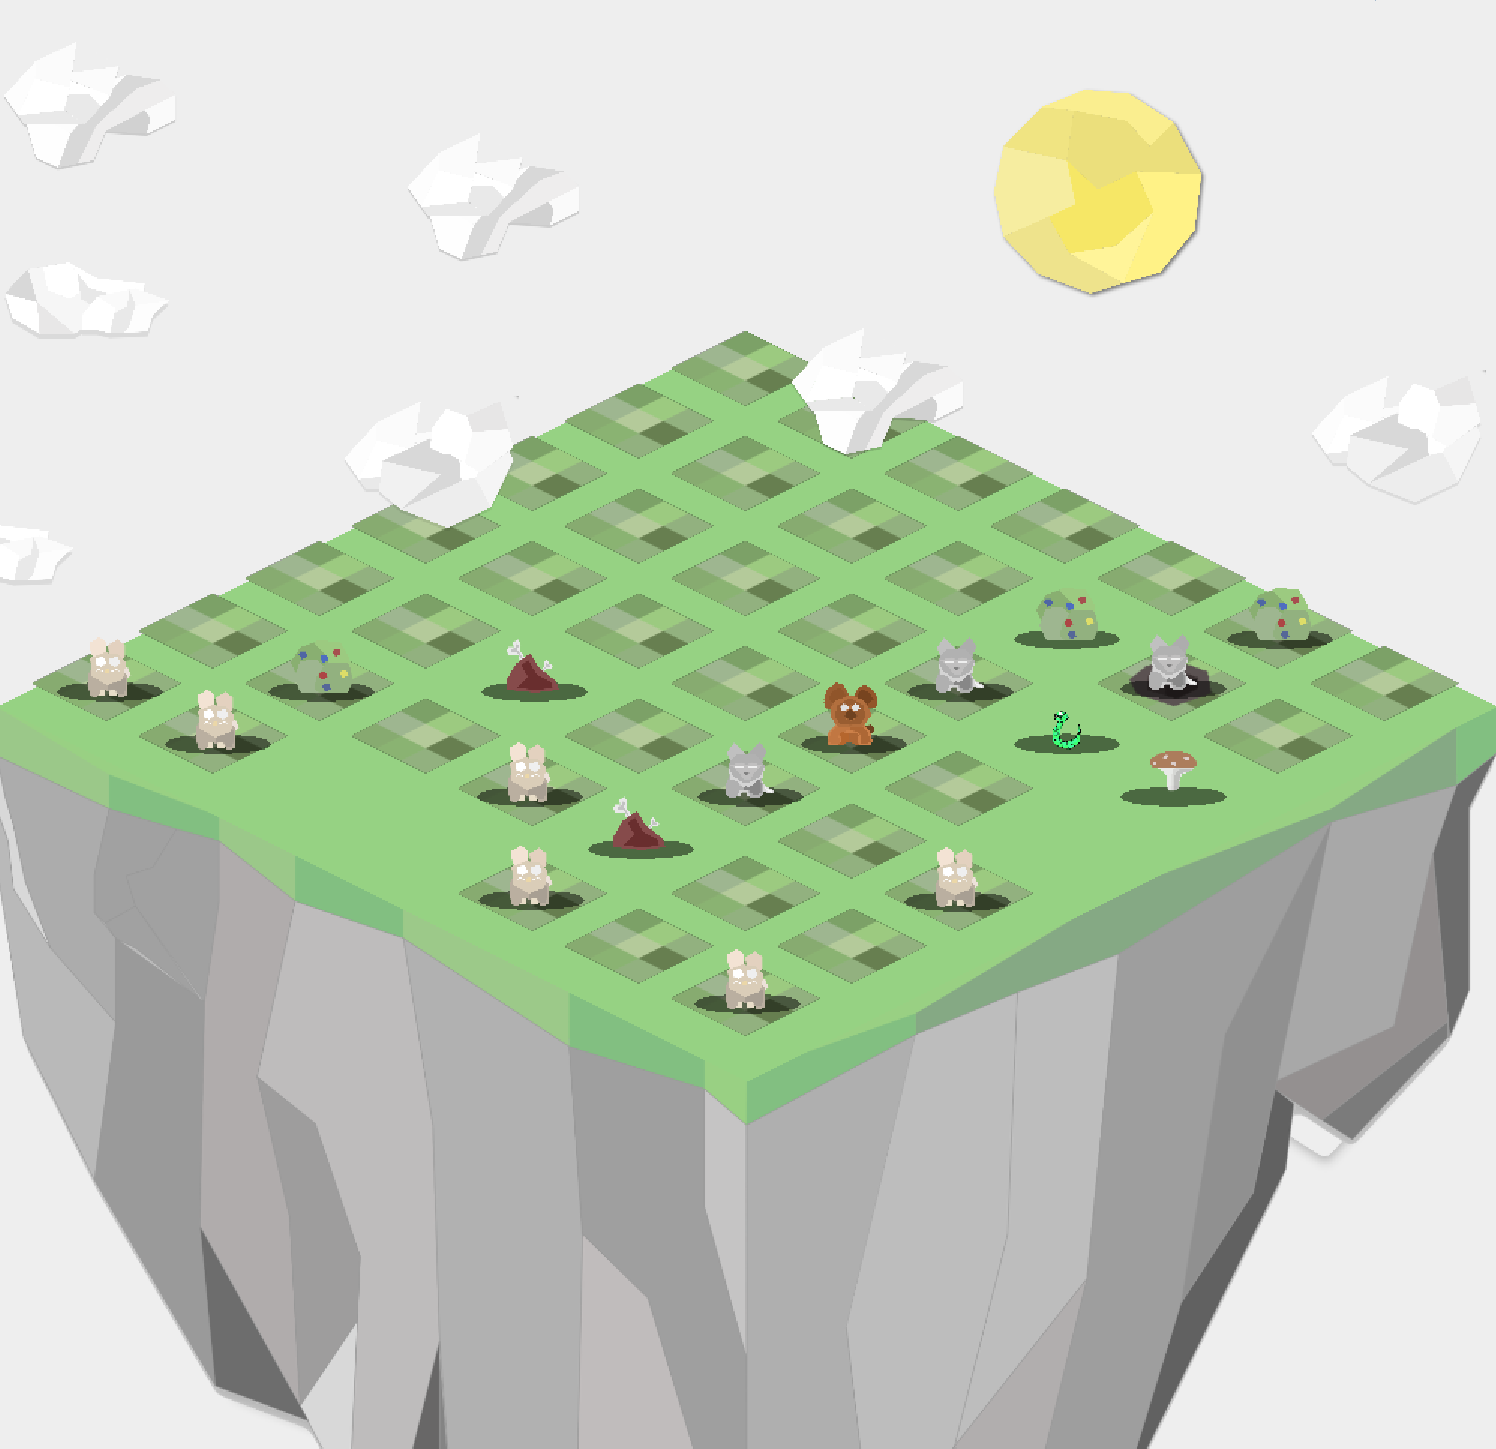
\includegraphics[width=.7\textwidth]{./screenshot.png}

    \vfill

    % University and date information at the bottom of the titlepage.
    IT-Universitetet i København\\
    Grundlæggende programmering \\
    BSGRPRO1KU\\
    21-12-2023 \\
    Antal anslag: 14287 \\
\end{titlepage}

\renewcommand{\contentsname}{Indholdsfortegnelse}
\tableofcontents
\newpage
    \section{Introduktion}
    Vi har fået til opgave at implementere og designe et økosystem, med brug af det udlevet biblioteket “ITUmulator”. Økosystemet udgøres af dyr, planter og svampe. Disse livsformer skal i sammenspil simulere et virkeligt økosystem, hvor dyr spiser, dør og reproducerer. Økosystemet har således en fødekæde, hvor nogle dyr fungerer som byttedyr, mens andre fungerer som rovdyr.
    \\Vi fik udleveret et bibliotek, ITUmulator, som vi skulle basere programmet på. ITUmulator stod for det grafiske, og biblioteket havde i forvejen implementeret et dag/nat-system, samt en metode, hvortil tiden bevæger sig fremad. Når programmet blev kørt, kørte simulationen derfor igennem en dag-nat-cyklus om og om igen. Vores opgave var at sørge for at der blev implementeret livsformer med forskellig opførsel, hvilket kunne skabe et virtuelt økosystem, som kunne sammenlignes med et økosystem fra virkeligheden. 
    \section{Design}
    En digital simulation af et økosystem, kan opbygges og designes på mange måder. Dette er også gældende for vores projekt, og vi har derfor været igennem mange design problematikker og beslutninger.
    \subsection{Inputfiler}
    Hver uge under projektet, er der blevet givet forskellige input-filer, som indeholdte start kriterier for økosystemet, det vil sige hvilke organismer der skulle starte i verdenen. Fra første uge, har håndteringen af input-filerne været et gennemløbende arbejdsområde, med mange iterationer. De første par uger var indlæsningen af input-filerne uoverskuelige og ikke skalerbar, da kravene for næste uge ikke var kendte. Derfor var indlæsningen af input-filerne meget statiske, indtil vi valgte at lave et helt nyt design til vores indlæsning. Omskrivningen blev gjort for at migrere til brug af “Java Reflection”.
    \\Med Java Reflection var det muligt at få programmets klasser til at konstruere, ændre og manipulere sig selv på runtime. Dette betød at det var muligt at konstruere en konstruktør til en klasse, hvor det derefter var muligt at initialisere klassens konstruktør med parameter fra input filerne på runtime. Denne løsning gjorde indlæsningen af input-filerne mere dynamiske, som løste komplikationerne med skalerbarheden. 
    \begin{figure}[H]
        \centering
        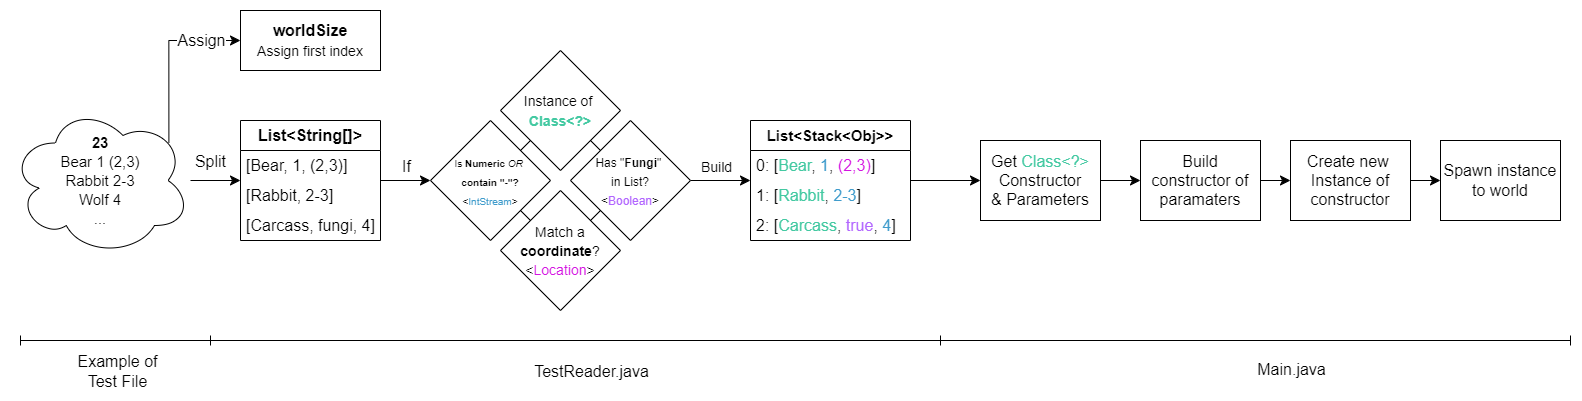
\includegraphics[width=1\columnwidth]{../TestReader.png}
        \caption{Flowchart eksempel af indlæsning, data repræsentation og konstruktør konstruktion af input fil.}
    \end{figure}
    \newpage
    \subsection{Vores organismer i økosystemet}I vores verden har vi fire dyr, en ulv, en bjørn, en slange og en kanin. Dyrene har mange fællestræk, de bevæger sig alle rundt på kortet, og når de er sultne, vil de lede efter mad at spise. Hvis et dyr ikke får nok mad eller hvis de bliver for gamle dør de. Når et dyr dør, vil den efterlade et ådsel, som andre rovdyr kan spise.
    Alle dyr kan enten være mætte, sultne (Hungry) eller sultende (Starving), hvis et dyr er ved at sulte, kan det finde på at gøre mere risikable eller drastiske handlinger.
    Alle dyr vil sove om natten, nogle i deres huler og andre i det åbne.
    Rovdyrene vil angribe andre dyr for at kunne spise dem. Mens byttedyr vil prøve at undgå rovdyrene.
    \\ 
    \\
    Nogle af dyrene har forskellige egenskaber, som er specifikke til dette dyr.
    En bjørn har et territorium som den helst ikke bevæger sig ud fra, men det kan ske, hvis den er sulten nok, at den vil bevæge sig væk fra sit territorium. Bjørnen er meget beskyttende over for sit territorium og vil angribe alt der kommer ind. Udover at spise kød spiser bjørnen også bær fra buske.
    En ulv angriber ikke bjørne alene, i stedet vil flokken sammen angribe en bjørn hvis de sultne.
    En kanin bor i huler om natten. Kaniner vil også prøve at undgå rovdyr ved at bevæge sig væk fra dem. Kaniner vil reproducere, hvis de støder ind i andre kaniner.
    Når en slange angriber, gør den ikke meget skade, i stedet vil den forgifte dyret. Et forgiftet dyr vil tage skade hen over tid. Slangen er det eneste dyr, der lægger æg. Når to slanger møder hinanden, kan de lægge et æg. Ægget vil efter noget tid klække og en babyslange vil komme ud.
    \\
    \\
    Ulvene fungerer som flokdyr. De har derfor en ulveflok. Ulveflokken har en leder ulv (eller en alfa-ulv). Lederen bliver valgt efter den stærkeste ulv i flokken og hvis en anden ulv bliver stærkere end lederen vil den blive valgt som den nye leder. Lederen sørger for at ulveflokken har en hule at bo i når det er nat. Det er ulveflokken, der står for at ulve parrer sig i deres huler om natten. Alle ulvene i ulveflokken bevæger sig ud fra hvor lederen bevæger sig. Når en af ulvene vælger at spise fra et ådsel, vil den dele maden med hele flokken, så alle i flokken får lidt mad, mens den specifikke ulv, der valgte at spise, vil få en smule mere.
    \\
    \\
    Udover dyrene har vi også mad, dyrene kan spise. Vi har tre forskellige slags mad, ådsler, græs og bærbuske.
    Ådsler opstår når et dyr dør, ådslet har en størrelse alt efter dyret der døde. Et ådsel bliver nedbrudt efter noget tid. Alle rovdyr spiser ådsler.
    Svampe kan opstå i et ådsel og svampe kan sprede sig fra ådsel til ådsel.
    Græs spreder sig når det dag. Dyr kan stå oven på græs. Græs er kaniners føde.
    Til sidst har vi buske, når det er dag, vil buskene forme bær, disse bær kan så blive spist af bjørne. Når bær er blevet spist vil der efter noget tid forme sig nye bær på busken.
    \newpage
    \subsection{Klassehierarki}
    Selve programmet består af 13 klasser, hvoraf to er abstrakte og et interface. Derudover bruger vi også tre interfaces fra biblioteket.
    \begin{figure}[H]
        \centering
        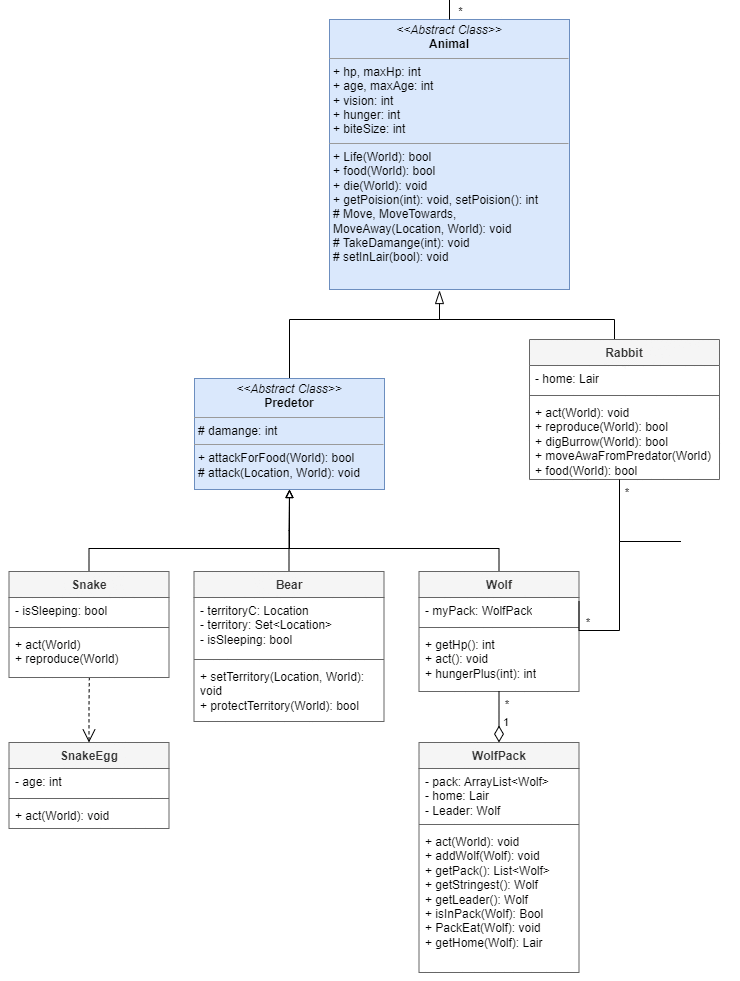
\includegraphics[width=0.5\columnwidth]{../ClassAnimal.png}
        \caption{Udsnit af klassediagrammet for Animal klasserne}
    \end{figure}
    Vi starter med at kigge på de 6 klasser, der handler om dyrene. Øverst har vi en overordnet abstrakt klasse “Animal” der er alle dyrs superklasse. Denne klasse står for alt som dyrene har tilfælles, blandt andet sult, alder, helbred, muligheden for at tage skade og at dyrene kan finde mad samt dø og bevæge sig.
    \\Tre ud af fire af vores dyr spiser kød og er derfor et rovdyr, vi har derfor en abstrakt klasse, “Predator”, der nedarver fra  superklassen “Animal”, som står for alt det rovdyr har tilfælles. Blandt andet at angribe andre dyr, finde dyr at angribe og hvor meget skade dyret gør.
    Ulv, bjørn og slange nedarve alle fra “Predator”, hvor kanin nedarver direkte fra “Animal”.
    \\Vi har en klasse “SnakeEgg” som bruges når slanger lægger æg, når en slange lægger et æg vil den initialisere et nyt æg som bliver vist på kortet og når ægget klækker vil den initialisere en ny slange.
    \newpage
    \begin{figure}[H]
        \centering
        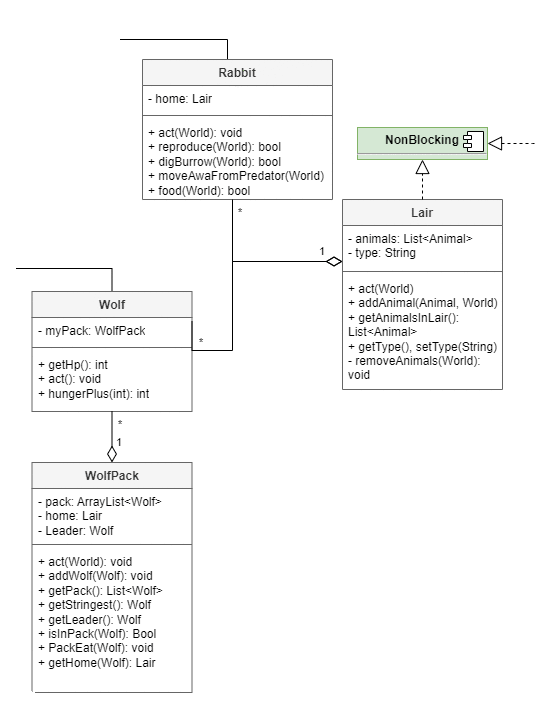
\includegraphics[width=0.4\columnwidth]{../ClassLair.png}
        \caption{Udsnit af klassediagrammet for Lair}
    \end{figure}
    To af vores dyr bor i huler om natten, vi har derfor en klasse “Lair” som står for alt hvad der har med hulen at gøre. Det vil sige når et dyr går ned i en hule er det denne klasse der står for det, samt sørger klassen også for at dyrene kommer ud af hulen når det bliver dag igen. Det er kaninen og ulven der bruger huler, klassen viser derfor en lille hule i verdenen hvis det en kaninhule og en stor hule i verdenen hvis det en ulvehule.
    \\For at holde styr på ulves flokke, har vi en klasse “Wolfpack”, denne klasse står for alt der har med en hel ulveflok at gøre. Blandt andet at de har en hule og at de kan formere sig i hulen. En ulv har en variable “Wolfpack” der holder styr på hvilken ulveflok den er en del af, og "Wolfpack", har en liste med alle ulve der er en del af denne ulveflok. En ulveflok har en leder ulv, “Wolfpack” har derfor en variable “Leader” som bliver sat til den ulv der er lederen af flokken.
    \begin{figure}[H]
        \centering
        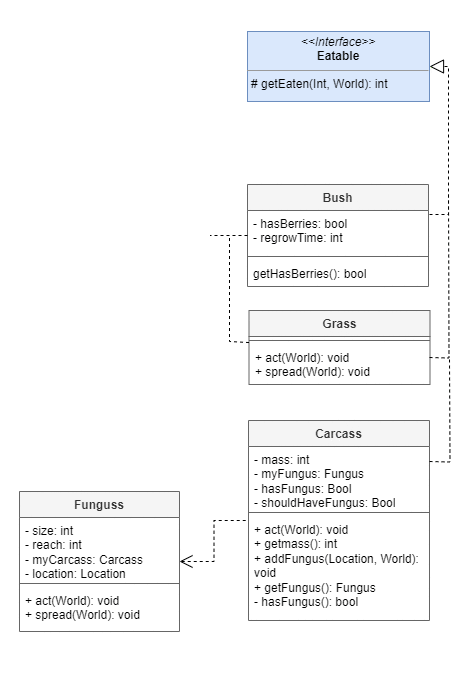
\includegraphics[width=0.4\columnwidth]{../ClassFood.png}
        \caption{Udsnit af klassediagrammet for Food klasser}  
    \end{figure}  
    Udover dyr, har vi tre typer af mad, til disse har vi et interface “Eatable” som alt der er mad implementerer. Dette interface sørger for at der bliver taget stilling til hvordan maden skal spises samt hvordan maden påvirker dyret.
    \\ \\I et ådsel kan der opstå en svamp, vi har derfor en klasse “Fungus” som sørger for at interagere med ådslet. Klassen “Fungus” og klassen “Carcass” er 2 individuelle klasser, men begge klasser har den modsatte type som variable så de nemt kan interagere med hinanden.
\\ \\Til sidst bruger vi også tre interfaces fra biblioteket ITUmulator.
“Non-blocking” er et interface der gør at noget kan være i  vores verden uden at blokere. Vi bruger det til græs og huler, så dyr kan stå og gå oven på græs og huler.
“Actor” er et interface der bruges til alle klasser der skal kunne interagere med vores verden, hvert step i vores simulation bliver en funktion “actor” kaldt på alle klasser der implementere interfacet. På denne måde kan vores dyr og planter interagere med vores verden.
Det sidste interface fra biblioteket er “DynamicDisplayInformationProvider” dette interface bruges visuelt til at vise vores organismer.
    \subsection{Behaviour}
    Vi valgte at det gav bedst mening, at et dyr kun kunne udføre én handling hvert step. På denne måde er det visuelt tydeligt, hvad der sker i verdenen, og dyrene har tid til at reagere på hinandens handlinger.
\\Derfor har vi opbygget den struktur der udgør dyrenes handling med en form for prioriteringsliste.
\\Først vil et dyr tjekke om det opfylder kravene til at udføre en af de prioriteter vi har givet. Hvis den gør det, vil den returnere i act metoden, hvilket gør at der ikke kan ske flere handlinger i det step. Hvis dyret ikke opfylder kravene om at udføre netop denne handling, vil den gå videre til den næstmest prioriterede handling. Dette fortsætter indtil dyret ikke kan gøre andet end at stå stille eller gå tilfældigt rundt, hvilket der er en halv halv chance for.
\\Nogle handlinger har en chance for at ske, hvis det ikke sker på grund af chancen, vil dyret også gå videre til næste prioritet.
\\Som eksempel kan vi se på Rabbit-klassen. Dens førsteprioritet er, at hvis den ikke har et hjem og den står på et kaninhul, vil den gøre dette til sit kaninhul. Da dette ikke kan ses i verdenen, har vi valgt at den gerne må lave en handling ud over dette, så her returneres der ikke. Dernæst tjekker vi kaninens alder, jo ældre den er, jo større chance er der for den ikke gør noget.
\\Dernæst er dens prioritet at rykke mod sit hjem, hvis det er nat. Hvis det ikke er nat, eller den ikke har et hjem, vil dette trin blive sprunget over, ellers vil der returneres, da kaninen nu har lavet en handling. Sådan fortsætter det igennem alle kaninens handlinger, indtil den finder en handling at udføre.
\begin{figure}[H]
    \centering
    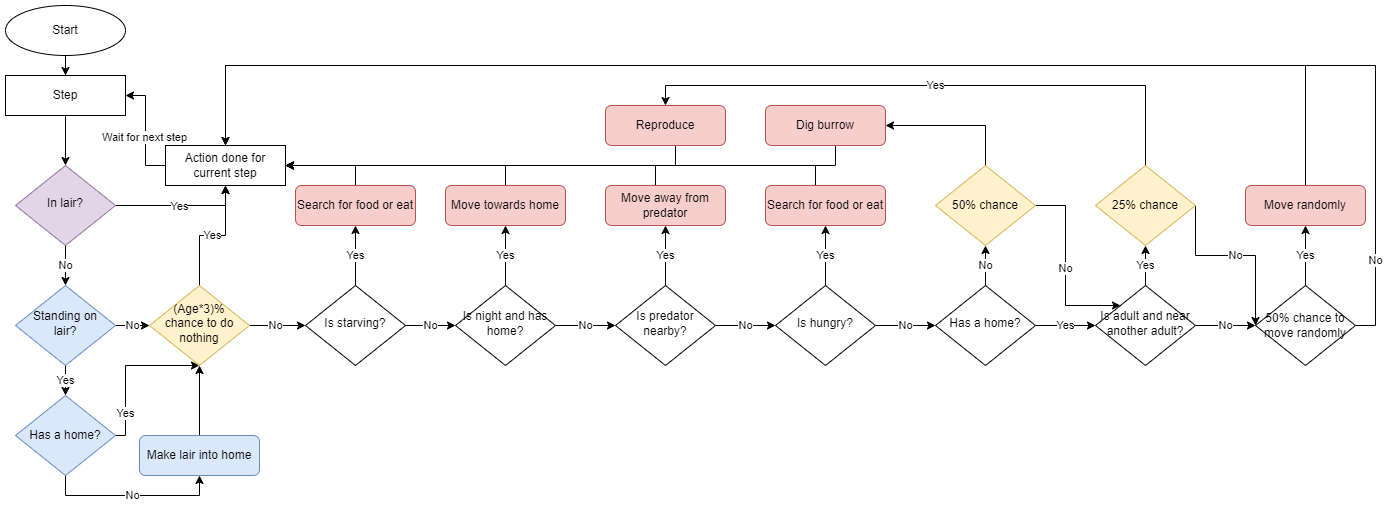
\includegraphics[width=1\columnwidth]{../BehaviourFlowchart.png}
    \caption{Flowchart af rabbit behaviour. Lilla er hvor der bliver tjekket om den sover, blå er en del af noget der bliver tjekker uden det tæller som en handling, gul er en vis \% chance og rød er handlinger.}  
\end{figure} 
Vi har valgt at bruge denne slags prioriteringsliste, da vi synes det lægger sig nært op af hvordan dyr opfører sig i naturen. For eksempel vil en sulten kanin nok altid lede efter mad, hvis den er sulten før den vil tænke på at reproducere. Dyr gør alting systematisk efter deres behov, de har ikke lyster på samme måde som mennesker og det synes vi denne form for prioriteringsliste løser godt.
Alle dyr kan enten være mætte, sultne (hungry) eller sultene (starving). Nogle handlinger forsøger dyret først at gøre, hvis det eksempelvis er starving. Det kan rykke på prioriteterne, så et dyr vil prioritere at spise eller lede efter mad, frem for at løbe væk fra et rovdyr. Når det kun er sulten, vil det prioritere andre ting, før dyret forsøger at spise, eller finde mad. Hvis et dyr er mæt, vil det ikke forsøge at hverken spise eller lede efter mad.
 \newpage  
\section{Testning}
    Projektets klasser og komponenter er blevet testet med brug af test automation, med brug af Unit-tests. Disse Unit-tests er Black-Box tests, hvor en klasses metoders output bliver testet i forhold til et givent kendt input. 
    \subsection{Fremgangsmåde for Test Driven Development}
    Igennem hele projektforløbet, har Test Driven Development (TDD) været brugt til at teste komponenterne i projektet. Normalt i TDD vil det være mest optimalt at skrive test cases før selve koden. Dette er for at sikre sig at alle elementer i projektet er testet, som gør programmet mere robust. 
    \\TDD var initiativet af projektforløbet til at starte med, men tidspres og andre komplikationer gjorde det svært at følge med. Individuelle test cases til hver mindre del af projektet gjorde det meget tidskrævende, da nye metoder til håndtering af samme logik hurtigt blev fundet. Dette gjorde at de gamle test cases blev hurtigt “outdated” og skulle omskrives eller fjernes. Udvikling af Unit-tests blev først rigtig implementeret igen til slut i projektforløbet, da det var mere overskueligt med projektets krav og gruppens egen fremgangsmåde.
    \subsection{Unit-tests \& kunstige økosystemer}
    Ved test af de forskellige krav, har ITUmulator bibliotekets opbygning gjort det anderledes at teste programmet og dens komponenter end normalt. ITUmulators brug af “Actor” interfacet og dens centralisering af logik i act()-metoden gør det svært at eksempelvis unit test mindre logik dele i act()-metoden. For at undgå dette problem, har vi lavet mange mindre metoder som individuelt kunne Unit-testes, som så blev brugt inde i act()-metoden. Det blev derfor valgt at lave størstedelen af metoderne “public” så de kunne unit testes. Udover at Unit teste individuelle metoder, har vi også lavet test til alle de individuelle krav. Dette blev gjort ved at kunstigt konstruere et økosystem og teste, om kravet kunne blive opfyldt. Dette kunne eksempelvis være om en kanin ville spise græs, hvis den var sulten. Hvis dette skulle testes, ville et kunstigt økosystem blive lavet, med kun en enkelt kanin og et stykke græs. De blev så testet, om kaninen ville spise græsset, og derved blive mere mæt og teste at græsset forsvinder efter.
    \section{Konklusion}
    Vi har igennem de sidste uger skabt en simulation af liv. Vi har lavet en “mini-verden”, der består af dyr, planter og svampe. Vi har lavet projektet baseret på et udleveret bibliotek, hvor vi skulle designe alle de forskellige aktører og deres handlinger. Vi skulle foretage designvalg, alt efter hvordan vi valgte at opfylde kravene. Vi har forsøgt at tage højde for, hvordan dyrene nogenlunde ville have opført sig i et virkeligt økosystem. Vi skulle overveje hvordan vi ville strukturere vores klasser, og hvordan vi bedst kunne udnytte objektorienteret programmering. Vores basale designfilosofi bag, hvordan dyrene opfører sig i forskellige situationer, er ved at gøre brug af en prioritetsliste. Programmet vil starte fra toppen, og bevæge sig ned i listen, hvor den tjekker, hvorvidt nogle krav bliver opfyldt, hvorefter den så vil udføre en enkelt handling. 
    \\Vi gjorde brug af JUnit tests, selvom vi lavede de fleste af vores endelige tests, da vi havde færdiggjort størstedelen af programmet. 
    \newpage
    \begin{landscape}
        \thispagestyle{empty}
        \section{Bilag}
    \begin{figure}[H]
        \centering
        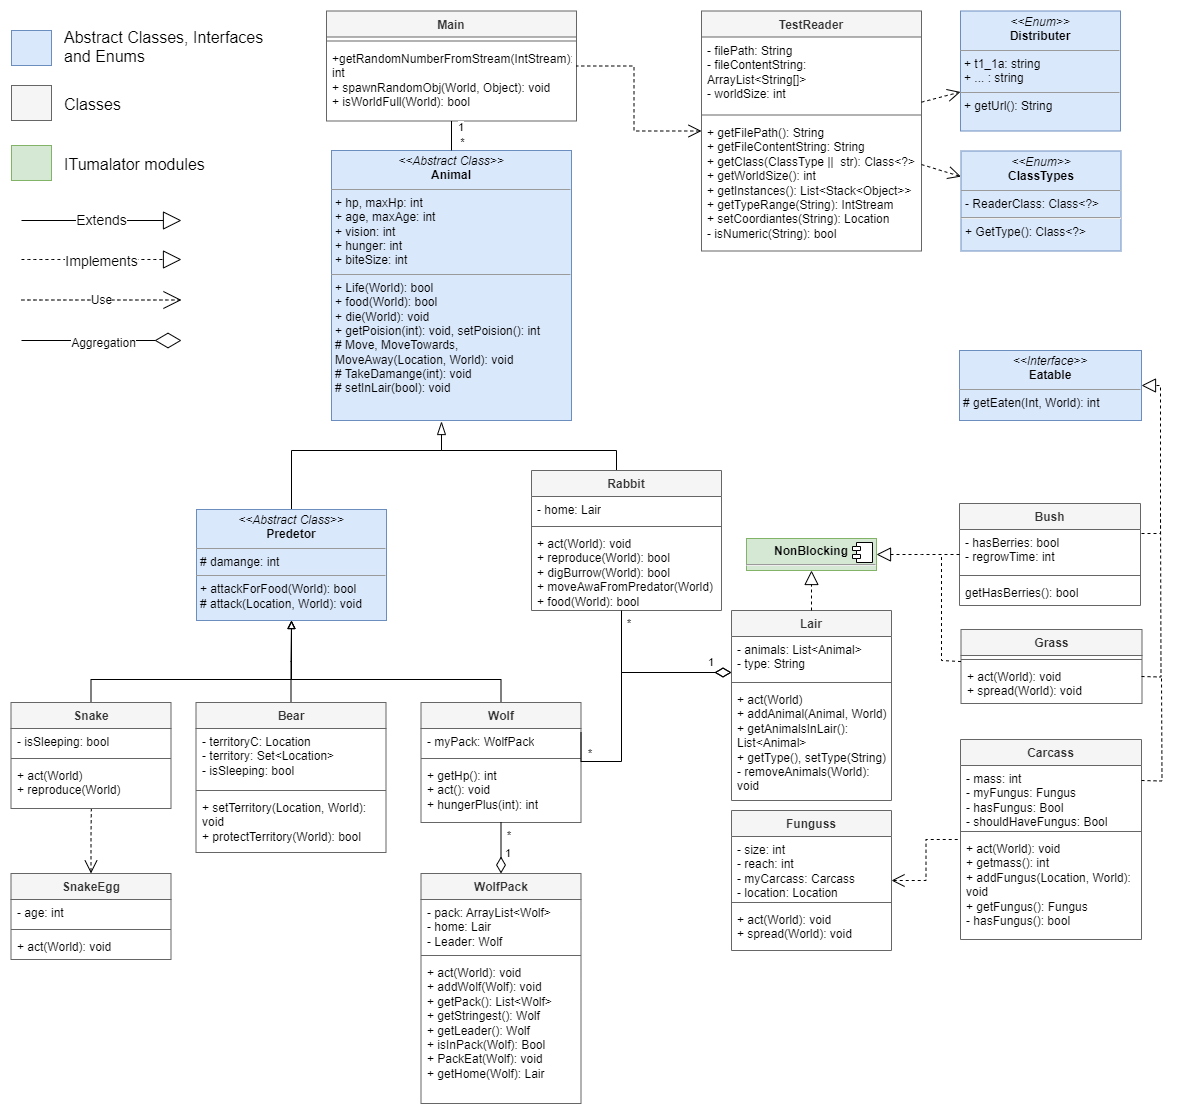
\includegraphics[width=0.6\columnwidth]{../ClassDiagram.png}
        \caption{Klasse Diagram for projektet}
    \end{figure}
    \end{landscape}
\end{document}
